% DSXL_3_doc_and_exercices_CREATION_DEVOIR.tex
\section{Structure des fichier CSV des devoirs}

La création d'un devoir commence par la création d'un fichier CSV qui sera placé dans l'un des sous répertoires de $données\_exercices$ :

\begin{verbatim}
 
./classe_3eme:
    2024_sem_09_3eme1.csv

./classe_seconde:
    2024_sem_25_2nd5.csv

./classe_terminale:
\end{verbatim}


 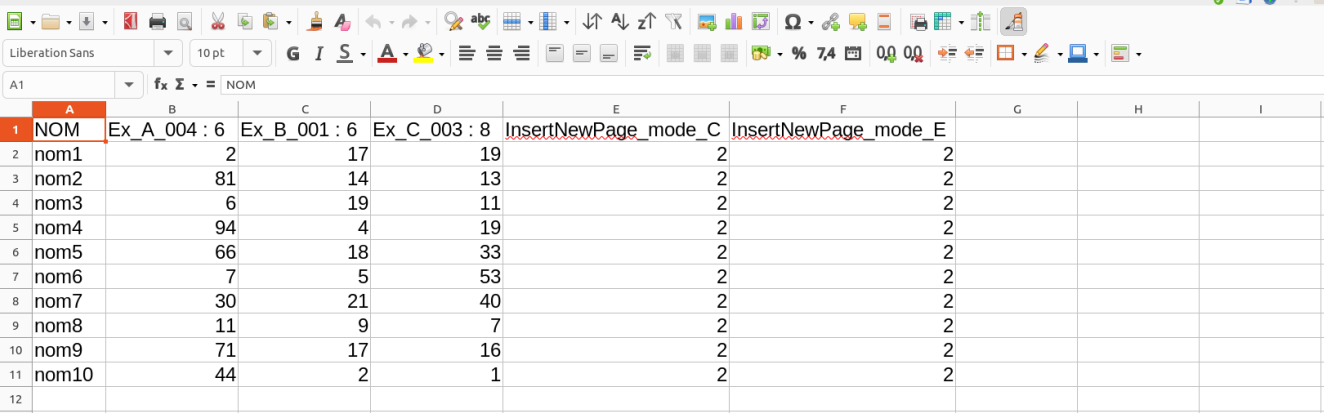
\includegraphics[width=15cm,height=6cm]{./images/creation_devoir_01.png}

La structure de ce fichier est simple : 

\begin{description}
 \item[1ere ligne : ] Cette 1ere ligne contient le nom des champs présents :
 \begin{description}
  \item[champs NOM : ] Cette colonne contient la liste des noms des élèves/étudiants
  \item[champs Numéros exercices : ] Ces champs sont définis de la manière suivante $Ex\_A\_001 : 6$ $=$ $Ex\_$(pour exercice) 
      $A$(numérotation de chaque colonne par lettre alphabétique) $ \_001$ (numéro de l'exercice)$ : 6$ (nombre de points pour l'exercice).
  \item[champs $InsertNewPage\_mode\_C$ \& $InsertNewPage\_mode\_E$ : ] Comme les énoncés des élèves sont mis les uns après les autres dans un grand fichier pdf, il est important de pouvoir  insérer un certain nombre de pages vides afin que pour chaque élève le corrigé (mode C) ou l'énoncé (mode E) ait un nombre pair de pages. 
Comme il y a parfois des effets de seuil, il est important de pouvoir individualiser ce nombre de pages pour chaque élève/étudiant. 
\end{description}
\item[Autres lignes : ] Elles contiennent les données relatives à chaque élèves. Le numéro sous chaque colonne commençant par $Ex\_$ contient le numéro de paramètre pour les valeurs numériques utilisés dans l'exercice pour l'élève/l'étudiant. 
\end{description}



\begin{dsxl}
 La numérotation de chaque colonne exercice n'est pas indispensable si tous les exercices utilisés sont différents. 
\end{dsxl}

\begin{bug}
 Si le fichier CSV est ouvert par un autre programme, comme par exemple LibreOffice, un fichier de vérouillage apparaît qui porte presque le même nom que le fichier ouvert \\ (par exemple $.\~ lock.2024\_sem\_25\_2nd5.csv\#$). Cela perturbe le programme et il faut fermer le fichier ouvert par l'autre application. 
\end{bug}

\section{Utilisation du programme $dsxl\_3\_devoir\_creation$}

Après démarrage du programme, on a l'ouverture d'une fenêtre avec deux onglets : \onglet{niveau/devoir} et \onglet{Devoirs : Paramètres}  



 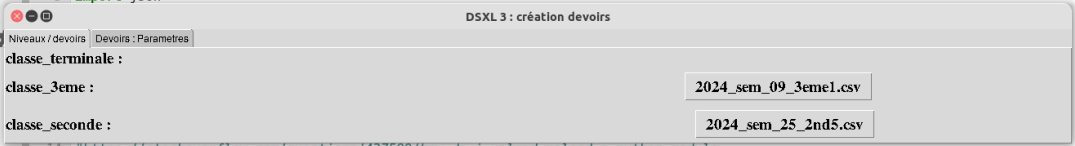
\includegraphics[width=15cm,height=2cm]{./images/creation_devoir_02.png}
 
\subsection{L'onglet \onglet{niveau/devoir}} 

 Le programme a repéré l'existence de deux fichiers (donc deux devoirs) CSV. Ils sont symbolisés par un bouton. 
 
 Choisissons le devoir $2024\_sem\_25\_2nd5.csv$ en cliquant sur le bouton $2024\_sem\_25\_2nd5.csv$. Il ne se passe rien, sauf peut-être un redimmensionnement de la fenêtre. 
 
 
 
Cliquons maintenant sur  l'\onglet{Devoirs : Paramètres} :

\subsection{L'\onglet{Devoirs : Paramètres}}

On obtient l'image suivante : 

 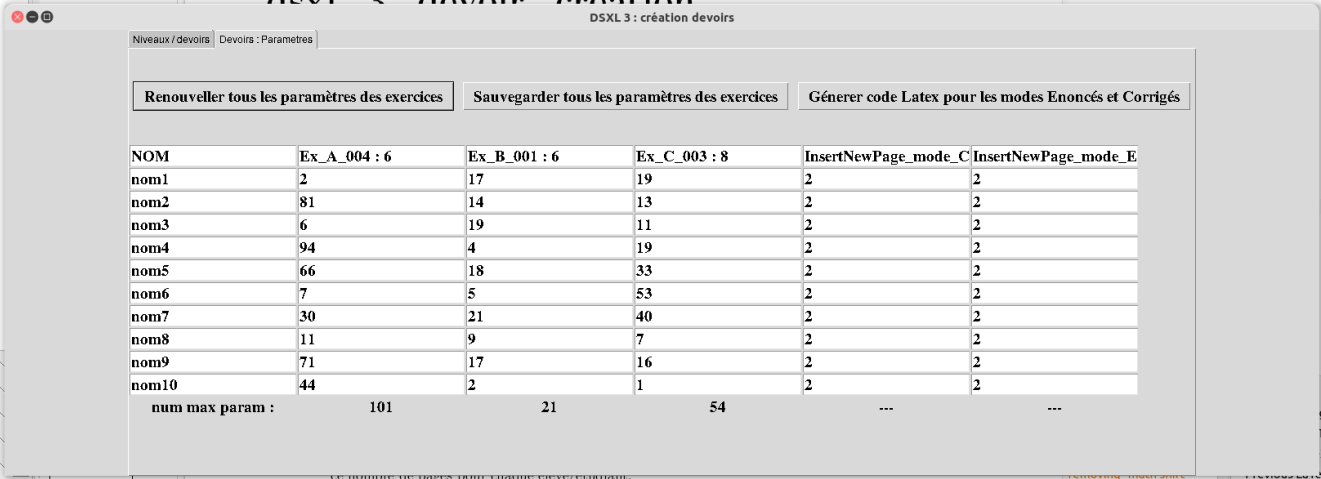
\includegraphics[width=15cm,height=8cm]{./images/creation_devoir_03.png}

On retrouve exactement le contennu du fichier CSV ouvert. 

De plus, une ligne supplémentaire apparaît tout en bas : elle contient le nombre maximum de variantes pour chaque exercice. 

Chaque entrée du tableau qui s'affiche peut être modifié à la main. Cela peut-être utile pour plusieurs raisons : 
\begin{enumerate}
 \item Des élèves ont la même variante d'exercice. 
 \item Un élève a une variante qui ne correspond pas à son niveau.
 \item On souhaite que deux élèves travaillent ensemble avec la même variante.  
\end{enumerate}

Trois commandes/boutons sont disponibles :

\begin{description}
 \item[Renouveler tous les paramètres des exercices : ] Il est possible de créér ainsi un nouveau devoir pour un rattrapage ou autre. Les valeurs générées sont aléatoires. 
 \item[Sauvegarder tous les paramètres des exercices : ] Permet de sauvegarder les valeurs du tableau dans le fichier qui a été choisi. 
 \item[Générer code Latex pour les modes énoncé (E) et corrigé (C) : ] Ces fichiers sont déposés dans les répertoires : 
 \begin{description}
  \item[$creation\_devoir/mode\_C$ : ] Il contiendra le corrigé de chaque exercice pour chaque élève.
   \item[$creation\_devoir/mode\_E$ : ] Il contiendra l'énoncé de chaque exercice pour chaque élève.
 \end{description}
 Ces fichiers sont complets et, normalement, peuvent être compilés sans problème. 
 
\end{description}

\begin{dsxl}
 Si les conventions sur le barême définies page \pageref{convention bareme question} ont été respectées, alors le mode 
 \begin{description}
  \item[ Correction (C) : ] donnera le barême question par question et
  \item[ Correction (E) : ] donnera le barême exercice par exercice et le nombre total de points. 
 \end{description}

\end{dsxl}


 
 
